%% Copernicus Publications Manuscript Preparation Template for LaTeX Submissions
%% ---------------------------------
%% This template should be used for copernicus.cls
%% The class file and some style files are bundled in the Copernicus Latex Package, which can be downloaded from the different journal webpages.
%% For further assistance please contact Copernicus Publications at: production@copernicus.org
%% https://publications.copernicus.org/for_authors/manuscript_preparation.html


%% Please use the following documentclass and journal abbreviations for preprints and final revised papers.

%% 2-column papers and preprints
\documentclass[journal abbreviation, manuscript]{copernicus}

\def\MM#1{\boldsymbol{#1}}
\DeclareMathOperator{\diff}{d}
\newcommand{\avg}[1]{\{#1\}}
\newcommand{\jump}[1]{[\![#1]\!]}
\newcommand{\pp}[2]{\frac{\partial #1}{\partial #2}} 
\newcommand{\JScomment}[1]{\textit{\textbf{Jemma says: #1}}}

%% Journal abbreviations (please use the same for preprints and final revised papers)


% Advances in Geosciences (adgeo)
% Advances in Radio Science (ars)
% Advances in Science and Research (asr)
% Advances in Statistical Climatology, Meteorology and Oceanography (ascmo)
% Aerosol Research (ar)
% Annales Geophysicae (angeo)
% Archives Animal Breeding (aab)
% Atmospheric Chemistry and Physics (acp)
% Atmospheric Measurement Techniques (amt)
% Biogeosciences (bg)
% Climate of the Past (cp)
% DEUQUA Special Publications (deuquasp)
% Earth Surface Dynamics (esurf)
% Earth System Dynamics (esd)
% Earth System Science Data (essd)
% E&G Quaternary Science Journal (egqsj)
% EGUsphere (egusphere) | This is only for EGUsphere preprints submitted without relation to an EGU journal.
% European Journal of Mineralogy (ejm)
% Fossil Record (fr)
% Geochronology (gchron)
% Geographica Helvetica (gh)
% Geoscience Communication (gc)
% Geoscientific Instrumentation, Methods and Data Systems (gi)
% Geoscientific Model Development (gmd)
% History of Geo- and Space Sciences (hgss)
% Hydrology and Earth System Sciences (hess)
% Journal of Bone and Joint Infection (jbji)
% Journal of Micropalaeontology (jm)
% Journal of Sensors and Sensor Systems (jsss)
% Magnetic Resonance (mr)
% Mechanical Sciences (ms)
% Natural Hazards and Earth System Sciences (nhess)
% Nonlinear Processes in Geophysics (npg)
% Ocean Science (os)
% Polarforschung - Journal of the German Society for Polar Research (polf)
% Primate Biology (pb)
% Proceedings of the International Association of Hydrological Sciences (piahs)
% Safety of Nuclear Waste Disposal (sand)
% Scientific Drilling (sd)
% SOIL (soil)
% Solid Earth (se)
% State of the Planet (sp)
% The Cryosphere (tc)
% Weather and Climate Dynamics (wcd)
% Web Ecology (we)
% Wind Energy Science (wes)


%% \usepackage commands included in the copernicus.cls:
%\usepackage[german, english]{babel}
%\usepackage{tabularx}
%\usepackage{cancel}
%\usepackage{multirow}
%\usepackage{supertabular}
\usepackage{algorithmic}
\usepackage{algorithm}
%\usepackage{amsthm}
%\usepackage{float}
%\usepackage{subfig}
%\usepackage{rotating}

\begin{document}

\title{Gusto: a toolkit for compatible finite element dynamical cores}

% \Author[affil]{given_name}{surname}

\Author[1,*]{Jemma}{Shipton}
\Author[2]{Thomas M.}{Bendall}
\Author[3]{So many}{Others}

\affil[1]{Department of Mathematics and Statistics, University of Exeter}
\affil[2]{Met Office}

%% The [] brackets identify the author with the corresponding affiliation. 1, 2, 3, etc. should be inserted.

%% If an author is deceased, please mark the respective author name(s) with a dagger, e.g. "\Author[2,$\dag$]{Anton}{Smith}", and add a further "\affil[$\dag$]{deceased, 1 July 2019}".

%% If authors contributed equally, please mark the respective author names with an asterisk, e.g. "\Author[2,*]{Anton}{Smith}" and "\Author[3,*]{Bradley}{Miller}" and add a further affiliation: "\affil[*]{These authors contributed equally to this work.}".


\correspondence{NAME (EMAIL)}

\runningtitle{TEXT}

\runningauthor{TEXT}





\received{}
\pubdiscuss{} %% only important for two-stage journals
\revised{}
\accepted{}
\published{}

%% These dates will be inserted by Copernicus Publications during the typesetting process.


\firstpage{1}

\maketitle



\begin{abstract}
TEXT
\end{abstract}

\begin{itemize}
\item Section 1: why compatible FEM
\item Section 2: why Gusto
\item Sections 3 and 4: this is Gusto
\item Section 5: and here are some examples of what we can currently do
\end{itemize}

\introduction   %% \introduction[modified heading if necessary]

\subsection{Motivation}
\begin{itemize}
\item many choices and research to be done - Colin says so in his Acta Numerica paper! - therefore flexible implementation is useful
\end{itemize}

Compatible finite element methods provide a route to stable,
consistent discretisations of the partial differential equations
governing geophysical fluids \citep{cotter2023compatible}. They
possess many of the desirable properties described by
\citet{staniforth2012horizontal} as essential for the accuracy of the
dynamical core of weather and climate models, such as conservation of
mass (and potentially other quantities such as energy and enstrophy),
correct wave propagation speeds and avoidance of spurious
computational modes, even on non-orthogonal grids. Obtaining these
properties on a non-orthogonal grid is important because weather and
climate models achieve optimal performance on supercomputers by
performing calculations concurrently, or in parallel, and orthogonal
grids of a spherical manifold will necessarily have singular points
that lead to a degredation in parallel scaling. An example of this is
the commonly-used latitude-longitude grid where the singular points
are the poles.

% In practice, this means that the spatial domain is partitioned into
% subdomains that are shared across the processors and data on the
% boundaries of the subdomains needs to be shared between the
% processors to compute a global solution. Current trends in
% supercomputer architectures
% are run on massivly parallel supercomputers that require the co
% Spatial domain decomposition methods share the computation
% across processors by

While the required properties of the discretisation guide the choice
of finite element spaces, there are many options for both the spatial
and temporal discretisation and it is not clear which will be best for
any particular problem. Gusto provides a flexible, extensible,
easy-to-use toolkit of options for rapid prototyping of different
spatial and temporal discretisations based on the compatible finite
element framework applied to geophysical fluid dynamics equations
relevant to numerical weather and climate prediction. In this paper we
introduce Gusto to the community, summarise its current capabilities
and outline our vision for future development.

\subsection{Background}

\begin{itemize}
\item overall theory is described in \citet{gibson2019compatible, cotter2023compatible}
\item Gusto has grown out of code described in \citet{natale2016compatible, cotter2012mixed, bendall2019recovered, bendall2020compatible, yamazaki2017vertical, shipton2018higher}
\item links to LFRic - we mention the Gung Ho project on the Gusto website so should describe that link here
\end{itemize}

The finite element method represents fields (e.g. velocity, pressure,
density or temperature) on a mesh made of non-overlapping, conforming
cells, or elements. Within each element, the field is represented as a
sum of coefficients multiplied by polynomial basis functions. The
finite element space is specified by the degree of the polynomial
basis functions and the continuity of these functions between the
elements. The partial differential equations used in weather and
climate modelling have multiple prognostic fields and it is not
necessary, or indeed desirable, to use the same finite element
representation for each field. Using different finite element
representations for each field gives what is known as a mixed finite
element discretisation.

`Compatible' or `mimetic' finite element discretisations are
constructed by choosing the different finite element representations
so that discrete versions of continuous vector calculus identities
hold. These methods are useful in a variety of applications due to
their ability to capture the underlying geometric structure of the
governing equations. In the context of geophysical fluid dynamics,
these methods are useful because they represent geostrophic balance
exactly which is crucial for reproducing accurate simulations of the
large-scale flow. In addition to this, there is flexibility within the
compatible finite element framework to choose representations that
also give other advantages such as energy conservation, local mass
conservation and discrete dispersion properties that lead to no
spurious pressure modes.

The compatible finite element spaces relevant for geophysical fluid
dynamics are constructed from a discrete differential complex called
the de Rham complex. This is a sequence of spaces with differential
operators between them that map onto the kernel of the next operator
in the sequence. This is often summarised in a commutation diagram as
in figures \ref{fig:2DdeRham} and \ref{fig:3DdeRham}. In these
diagrams the infinite dimensional spaces are along the top row and the
$\pi_i$ denote projections into the corresponding finite dimensional
subspace used in the compatible finite element discretisation. The
differential operators are denoted by $\diff^k$ and these commute with
the projections, meaning that $\diff^{k+1}\pi_k(\cdot) =
\pi_{k+1}\diff^{k+1}(\cdot)$. This guarantees that, in 3D, $\nabla$
maps onto the kernel of $\nabla\times$, ensuring
$\nabla\times\nabla(\cdot)=0$, and $\nabla\times$ maps onto the kernel
of $\nabla\cdot$, ensuring that $\nabla\cdot\nabla\times(\cdot)=0$;
i.e. the spaces are compatible. In 2D we have that $\nabla^\perp$
(the 2D curl operator) maps onto the kernel of $\nabla\cdot$,
ensuring that $\nabla\cdot\nabla^\perp(\cdot)=0$. It is possible to
write this de Rham complex such that instead $\nabla$ maps onto the
kernel of $\nabla^\perp$, ensuring that
$\nabla^\perp\cdot\nabla(\cdot)=0$, but the former is more useful in
constructing discretisations for geophysical fluid dynamics since it
enables schemes with local mass conservation \citep{}.

\begin{figure}
  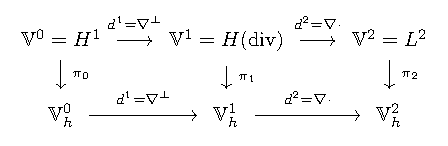
\includegraphics{figures/de_rham_fig_2d.pdf}
  \caption{De Rham complex for two dimensional spaces. The
    interelement continuity of the functions decreases from left to
    right, with functions in $\mathbb{V}^{H^1}$ being fully
    continuous, those in $\mathbb{V}^{HDiv}$ having continuous normal
    components and those in $\mathbb{V}^{L^2}$ being fully
  discontinuous. The polynomial order also decreases from left to
  right.}
  \label{fig:2DdeRham}
\end{figure}

\begin{figure}
  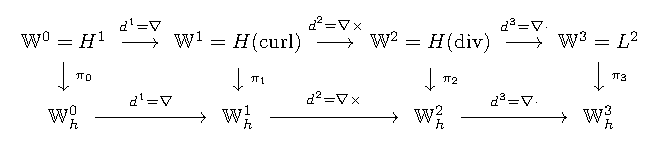
\includegraphics{figures/de_rham_fig_3d.pdf}
  \caption{De Rham complex for three dimensional spaces. The
    interelement continuity of the functions decreases from left to
    right, with functions in $\mathbb{V}^{H^1}$ being fully
    continuous, those in $\mathbb{V}^{HCurl}$ having continuous
    tangential components, those in $\mathbb{V}^{HDiv}$ having
    continuous normal components and those in $\mathbb{V}^{L^2}$ being
    fully discontinuous. The polynomial order also decreases from left
    to right.}
  \label{fig:3DdeRham}
\end{figure}

Due to these promising properties, the next Met Office dynamical core
will use the lowest order compatible finite element discretisation on
the cubed sphere \citep{}. However, there are many important avenues
for research and unanswered questions relating to, for example, the
choice of grid and $\mathbb{V}^{HDiv}_h$; the design of transport
schemes; stable and efficient timestepping algorithms; linear solver
techniques and how to couple unresolved physics processes to the
resolved dynamics. This type of research is difficult in operational
models, which are generally designed to execute specific
configurations very efficiently. The purpose of Gusto is to facilitate
this research by providing an open source, flexible, extensible
framework that provides the key components required when designing
algorithms for a dynamical core. These include: finite element
function spaces defined on the sphere (where the Piola transform is
required to... **); meshes that have a columnar structure (because**),
stable transport and diffusion schemes for variables with different
interelement continuity,



* In 3D the function spaces have a tensor product structure
* The function spaces are hard to construct especially on the sphere - piola transform, theta space

* Gusto has grown out of code developed in (see above refs)
* The idea is to bring together methods using compatible finite element discretisations in a well-tested and documented code base that can be extended and applied to different problems of interest to the community.
* X did Y - quick history of the development of the methods, plus others that are not actually in Gusto at the moment.

In this article we will describe the current capabilities of Gusto and
the design features that enable our flexible implementation whereby
different spatial and temporal discretisations can be applied to a
range of different equation sets relevant for weather and climate
modelling. In section \ref{sec: governing} we will outline three
different equation sets commonly used for modelling geophysical fluids
in order to demonstrate the similarities between the equation sets and
justify the use of a unified codebase. The advantages of this unified
approach become even clearer in section \ref{sec: FEM} where we
present the compatible finite element discretisation of the different
types of terms (e.g. pressure gradient, transport, diffusion) seen in
section \ref{sec: governing}. In section \ref{sec: design} we describe
the code structure of Gusto followed by a detailed example (section
\ref{sec: FML}) of the Form Manipulation Language (FML) that
facilitates symbolic manipulation of the finite element forms within
our timestepping code. Section \ref{sec: results} contains a selection
of numerical results that showcases the range of discretisations
available within Gusto. We summarise our current status and future
directions in section \ref{sec: summary}.

\section{Governing Equations}
\label{sec: governing}
The aim of this section is to introduce three governing equation sets
commonly used in the development of discretisation methods for weather
and climate models, along with enough detail about the finite element
discretiations provided by Gusto to demonstrate the similarities
between them. These similarities guide the design of the code
structure described in the next section and motivate the use of Form
Manipulation Language (FML) that underlies the flexibility of Gusto, a
detailed example of which will be given in section \ref{sec: FML}. The
convention in Gusto is to write the equations in residual form,
meaning that all the terms appear on the left side. We will follow
this convention below in contrast to many papers which present the
equations with the pressure gradient term and any forcing terms on the
right side.

\subsection{Shallow Water Equations}
The shallow water equations are commonly used for testing numerical
algorithms and for exploring geophysical fluid dynamics concepts under
simplified conditions. They are useful in both contexts since they are
the simplest set of equations that model motion on both the slow,
geostrophic timescale and the much faster timescale of the
inertia-gravity waves. This timescale separation poses challenges to
the numerical discretisation and also provides a rich enough range of
dynamics to explain many of the phenomena observed in the atmosphere
and oceans \citep{zeitlin2018geophysical}.

The shallow water equations describe the flow of a shallow layer of
fluid subject to gravitational and, optionally, rotational forces. The
prognostic variables are the two horizontal velocity components
$\MM{u} = (u, v)$ and the fluid depth $D = H + h - b$ where $H$ is the
undisturbed depth of the fluid layer, $h$ is the free surface
deviation from $H$, and $b$ is the bottom topography, if present. The
equations are:

\begin{align}
  \pp{\MM{u}}{t} + (\MM{u}\cdot\nabla)\MM{u} + f\hat{\MM{k}}\times\MM{u} + g\nabla (D+b) &= 0, \\
  \pp{D}{t} + \nabla\cdot(D\MM{u}) &= 0,
\end{align}
where $f$ is the Coriolis parameter, $\hat{\MM{k}}$ is the unit vector
pointing upwards and $g$ is the acceleration due to gravity.

\subsection{Compressible Boussinesq Equations}
The compressible Boussinesq equations are commonly used in ocean
modelling. They are useful from a numerical discretisation perspective
because they incorporate compressibility effects without the
complexity of discretising the nonlinear pressure gradient terms that
we shall see in the compressible Euler equations. We write these
equations in terms of the prognostic variables $\MM{u}$, $b$ and $p$
where $\MM{u}$ is the velocity field, $p$ is pressure and $b$ is the
fluid buoyancy. In terms of these variables, the equations are:

\begin{align}
  \pp{\MM{u}}{t} + 
  (\MM{u}\cdot\nabla)\MM{u} +
  2\MM{\Omega}\times \MM{u} + \nabla p + b\hat{\MM{k}} & = 0, \\
  \pp{p}{t} + c^2\nabla\cdot\MM{u} & = 0, \\
  \pp{b}{t} + (\MM{u}\cdot\nabla) b & = 0,
\end{align}
where $\MM{\Omega}$ is the rotation vector of the domain,
$\hat{\MM{k}}$ is the unit vector pointing upwards and $c$ is the
acoustic wave speed. The equations describe the motion of a
three dimensional stratified fluid but can also be solved in a
two dimensional vertical slice domain described by $(x, z)$
coordinates. In this case, the velocity $\MM{u}$ can either be
two dimensional as well (if there is no Coriolis force), or fully
three dimensional but with each Cartesian component only varying in
the $x-z$ plane. In the latter case, this is implemented using a
three dimensional computational domain that is only one element wide
in the $y$-direction and with periodic boundary conditions also in
that direction.

\subsection{Compressible Euler Equations}
The dynamical core at the heart of any weather or climate model solves
the rotating compressible Euler equations that model atmospheric
flow. We write these equations in terms of the prognostic variables
$\MM{u}$, $\rho$ and $\theta$ where $\MM{u}$ is the velocity field,
$\rho$ is the fluid density and $\theta$ is the potential
temperature. The pressure gradient term is written in terms of the
Exner pressure $\Pi$ which is calculated through an equation of
state. In terms of these variables, the equations are:

\begin{align}
  \pp{\MM{u}}{t} + 
  (\MM{u}\cdot\nabla)\MM{u} +
  2\MM{\Omega}\times \MM{u} + c_p\theta\nabla \Pi + g\hat{\MM{k}} & = 0, \\
  \pp{\rho}{t} + \nabla\cdot(\MM{u}\rho) & = 0, \\
  \pp{\theta}{t} + (\MM{u}\cdot\nabla)\theta & = 0, \\
  \Pi^{(1-\kappa)/\kappa} & = \frac{R}{p_0}\rho\theta, & 
\end{align}
where $\Pi$ is the Exner pressure, $p_0$ is a reference pressure, $R$
is the gas constant, $c_p$ is the specific heat at constant pressure
and $\kappa=R/c_p$. Again, these equations describe the motion of a
three dimensional stratified fluid but can also be solved in a
two dimensional vertical slice domain described by $(x, z)$
coordinates. In this case, the velocity $\MM{u}$ can either be two
dimensional as well (if there is no Coriolis force), or fully three
dimensional but with each Cartesian component only varying in the
$x-z$ plane. In the latter case, this is implemented using a three
dimensional computational domain that is only one element wide in the
$y$-direction and with periodic boundary conditions also in that
direction. \JScomment{I know this repeats what is said above but I
  like that each section is self-contained - I hope that is ok but
  also happy to change it!}

In all of the equation sets described here, the nonlinear velocity
advection term $(\MM{u}\cdot\nabla)\MM{u}$ can be replaced by the sum
of a vorticity-based term and the gradient of the kinetic energy. This
is known as the vector invariant form and it enables the construction
of schemes that conservation energy and/or enstrophy
\citep{mcrae2014energy, bauer2018energy, wimmer2020energy,
  wimmer2021energy}. However, this form can exhibit numerical
instabilities \citep{bell2017numerical} and it is not yet clear which
form is preferable so in Gusto we offer both forms of the equations.

\section{Finite Element Discretisation}
\label{sec: FEM}

Comparing the equation sets given in the previous section, we see
several similarities. For example, the prognostic equation for the
velocity always contains a nonlinear transport term, a term due to
rotation and a `pressure' gradient term (in shallow water this is the
gradient of the depth but the term plays the same role in the dynamics
and is derived from the pressure gradient term in the full equations
\citep{zeitlin2018geophysical}). The other prognostic fields satisfy
either an advective or continuity form of the transport
equation. These similarities remain when we formulate the compatible
finite element discretisations, as we shall see below, and importantly
this means that the discretisation of these terms can be written and
implemented in software so that it can be applied to any of the
equation sets.

The finite element discretisation is formed by choosing appropriate
representations, or function spaces, for the prognostic variables,
multiplying by test functions from these function spaces and
integrating over the domain. In addition to this, we integrate by
parts when the interelement continuity of the basis functions is not
sufficient to define the result of applying the differential operator
directly. For the domains considered in this paper, the only boundary
conditions we use are those of no normal flow, $\MM{u}\cdot\MM{n}=0$
where $\MM{n}$ is the outward pointing normal to the boundary. This
means that the test function for the velocity must also be chosen from
a function space that has this boundary condition.

In line with the theory outlined in the introduction, we always choose
the velocity $\MM{u} \in \ring{\mathbb{V}}^{HDiv}$ with
$\ring{\mathbb{V}}^{HDiv} \subset \mathbb{V}^{HDiv} \subset
H(\text{div})$ and, as mentioned above, the $\ring{}$ indicates that
the functions in $\ring{\mathbb{V}}^{HDiv}$ satisfy the no normal flow
boundary conditions. The field whose gradient appears in the
`pressure' gradient term is chosen to be in the space
$\mathbb{V}^{L^2}$ with $\mathbb{V}^{L^2} \subset L_2$, or, in the
case of the more complex nonlinear pressure gradient term for the
compressible Euler equations, it is a function of a variable in this
space. The compressible Boussinesq and compressible Euler equations
have a third prognostic variable, either buoyancy or potential
temperature, which is chosen to be in the space $\mathbb{V}_\theta$
which has degrees of freedom that are collocated with those of the
vertical velocity, mimicking the Charney-Phillips staggering as
discussed in **. These choices are governed by the properties required
of discretisation of the linearised equation sets (as discussed in
section ** and other refs). To solve the nonlinear equation sets we
need to introduce stable and accurate discretisations of the transport
terms and the nonlinear pressure gradient term in the compressible
Euler equation set. In addition, some test cases require viscous and
diffusive terms to generate converged solutions \ref{}. In the
following subsections we illustrate a non-exhaustive selection of the
options available in Gusto.

\subsection{Pressure gradient term}
The pressure gradient term is discretised in a similar way for each
equation set, with some additional considerations required for the
nonlinear form of this term in the compressible Euler equations. Since
the pressure (or depth, for shallow water) field is discretised in
$\mathbb{V}^{L^2} \subset L_2$, meaning that it is discontinuous between
cells, the gradient is not defined globally and the term must be
integrated by parts. In the linear case, using the notation for the
compressible Boussinesq equations, the weak form is

\begin{equation}
\int_\Omega\MM{w}\cdot\nabla p \diff x = -\int_\Omega\nabla\cdot\MM{w}p\diff x, \quad \forall \MM{w} \in \ring{\mathbb{V}}^{HDiv},
\end{equation}
where $\Omega$ denotes the domain and there are no surface terms from
the integration by parts because these vanish on interior element
boundaries since the normal component of $\MM{w}$ is continuous across
element facets and on exterior boundaries we set no normal flow
boundary conditions. However, the pressure gradient term in the
compressible Euler equations, $c_p\theta\nabla\Pi$, is nonlinear and
this introduces an additional complication. Integration by parts is
still required since $\Pi$ is evaluated as a function of the density
$\rho \in \mathbb{V}^{L^2}$ and $\theta \in \mathbb{V}_\theta$ so is
discontinuous between elements, but then integrating by parts
transfers the differential operator to $\MM{w}\theta$ which is
discontinuous in the horizontal direction. Following \ref{} we integrate by parts
in each element $e$, giving

\begin{equation}
  c_p\int_e\MM{w}\cdot\theta\nabla\Pi\diff x = -c_p\int_e\nabla\cdot(\MM{w}\theta)\Pi\diff x + c_p\int_{\partial e}\hat{\theta}\MM{w}\cdot\MM{n}\hat{\Pi}\diff S, \quad \forall \MM{w} \in \ring{\mathbb{V}}^{HDiv},
\end{equation}
where $\partial e$ denotes the element facets, $\MM{n}$ is the outward
pointing normal to the facet and $\hat{q}$ denotes the value of a
variable $q$ on the facet, which for discontinuous variables does not
have a unique definition. Summing over the domain gives

\begin{equation}
  c_p\int_\Omega\MM{w}\cdot\theta\nabla\Pi\diff x = -c_p\int_\Omega\nabla\cdot(\MM{w}\theta)\Pi\diff x + c_p\int_{\Gamma_v}\jump{\theta\MM{w}\cdot\MM{n}}\avg{\Pi} \diff S, \quad \forall \MM{w} \in \ring{\mathbb{V}}^{HDiv},
\end{equation}
where $\Gamma_v$ denotes the vertical element facets, across which
$\theta$, and therefore $\Pi$, are discontinuous. Here we have chosen,
as in \citet{}, to take the average value of $\Pi$ across the facets,
$\avg{\Pi} = (\Pi^++\Pi^-)/2$, where the $+$ and $-$ indicate each
side of the facet. The brackets $\jump{q} = q^+-q^-$ denote the jump
in $q$ across the facet and the integral over the horizontal facets
vanishes since both $\theta$ and $\MM{w}\cdot\MM{n}$ are continuous
across these facets so the jump is zero.

\subsection{Transport terms}
Since the prognostic variables are discretised using different finite
element function spaces $\mathbb{V}^{HDiv}$, $\mathbb{V}^{L^2}$ and
$\mathbb{V}_\theta$, each with different continuity properties between
the elements, the choice of stable transport discretisation is
different for each prognostic variable. The spatial order of the
finite element spaces also imposes requirements on the choice of
transport scheme. In particular, when the lowest order space
$\mathbb{V}^{L2}$ is chosen to be piecewise constant, we need to use
the recovered transport scheme described in
\citet{bendall2019recovered} to achieve second order convergence
overall. Here we describe the default transport schemes used in Gusto
for the next-to-lowest order sequence of function spaces (i.e. where
the lowest order space $\mathbb{V}^{L2}$ is chosen to be piecewise
linear and discontinuous between elements) and refer the reader to
\citet{bendall2019recovered} for details of the recovered schemes,
which are also implemented in Gusto.

\subsubsection{Transport of $\mathbb{V}^{L^2}$ fields}
The shallow water and compressible Euler equation sets both contain a
prognostic equation that is the continuity form of the transport
equation for a variable represented by a function that is fully
discontinuous between elements. This means that the divergence term is
not well defined. A stable discretiation of this equation can be
constructed by integrating that term by parts and taking the upwind
values on the element facets. Using the compressible Euler equation
notation, this gives, in each element $e$ with boundary $\partial e$:

\begin{equation}
  \int_e \phi\nabla\cdot(\rho\MM{u}) \diff x = -\int_e \nabla\phi \cdot (\rho\MM{u}) \diff x + \int_{\partial e} \phi\tilde{\rho}\MM{u}\cdot\MM{n} \diff S, \quad \forall \phi \in \mathbb{V}^{L^2}.
\end{equation}
Summing over the domain gives
\begin{equation}
  \int_\Omega \phi\nabla\cdot(\rho\MM{u}) \diff x = -\int_\Omega \nabla\phi \cdot (\rho\MM{u}) \diff x + \int_\Gamma \jump{\phi\MM{u}}\tilde{\rho} \diff S, \quad \forall \phi \in \mathbb{V}^{L^2},
\end{equation}
where $\Omega$ is the domain, $\Gamma$ denotes the element facets,
$\tilde{\rho}$ denotes the value of $\rho$ on the upwind side of the
facet and the brackets $\jump{q} = q^+-q^-$ denote the jump in $q$
across the facet.

\subsubsection{Transport of $\mathbb{V}_\theta$ fields}
The compressible Boussinesq and compressible Euler equation sets both
contain a prognostic equation that is the advective form of the
transport equation for a variable that is represented by a function
that is continuous in the vertical direction but discontinuous in the
horizontal direction. This means that the gradient of the field
required in the transport term is not well defined. A stable
discretisation of this equation can be constructed by using a
combination of the above upwinding strategy in the discontinuous
horizontal direction and a streamline-upwind Petrov-Galerkin (SUPG)
method in the continuous vertical dirction. The SUPG method replaces
the finite element test function $\gamma$ with $\gamma + \tau
\MM{u}\cdot\nabla\gamma$ where $\tau$ is a stabilisation parameter,
although here we just require the vertical part of the gradient term. This
has the effect of suppressing spurious oscillation associated with the
continuous finite element approximation of the transport term. The
stabilisation parameter $\tau$ depends on the spatial resolution and
** and is set to be ** by default in Gusto, following \citet{}.

We first integrate by parts in each column $C$ of the mesh, taking the
upwind value of the field, indicated by a $\tilde{}$, on the vertical
facets of the mesh, denoted by $\Gamma_v$. Using the notation of the
compressible Euler equations, this gives

\begin{align}
  \int_C \gamma\MM{u}\cdot\nabla\theta\diff x &= -\int_C \nabla\cdot(\gamma\MM{u})\theta \diff x + \int_{\Gamma_v}\gamma \MM{u}\cdot\MM{n}\tilde{\theta}\diff S, \quad \forall \gamma \in \mathbb{V}_\theta, \\
  &= \int_C \gamma\MM{u}\cdot\nabla\theta \diff x + \int_{\Gamma_v}\gamma \MM{u}\cdot\MM{n}(\tilde{\theta}-\theta_{int})\diff S, \quad \forall \gamma \in \mathbb{V}_\theta,
\end{align}
where we have integrated by parts a second time to move the
differential operator from $\gamma$ back to $\theta$ since we need to
replace the test function $\gamma$ with $\gamma+\tau w\gamma_z$, where
$w=\MM{u}\cdot\hat{\MM{z}}$ is the vertical component of the
velocity. This gives a second boundary term that now contains the
value of $\theta$ in the interior of the column, denoted by
$\theta_{int}$. Summing over the domain and applying the SUPG method
in the vertical gives
\begin{equation}
  \int_C \gamma\MM{u}\cdot\nabla\theta\diff x =\int_\Omega(\gamma+\tau w\gamma_z)\MM{u}\cdot\nabla\theta \diff x + \int_{\Gamma_v}\jump{(\gamma+\tau w\gamma_z) \MM{u}}\tilde{\theta}-\jump{(\gamma+\tau w\gamma_z) \MM{u}\theta}\diff S, \quad \forall \gamma \in \mathbb{V}_\theta.
\end{equation}
Note that, as explained in \citet{Colin}, the test function should
also be replaced in the time derivative term for consistency **
  

\subsubsection{Transport of $\mathbb{V}^{HDiv}$ fields}
All three of the equation sets described in section \ref{} include a
prognostic equation for the velocity field
$\MM{u}\in\mathbb{V}^{HDiv}$ that contains a nonlinear transport term
$\MM{u}\cdot\nabla\MM{u}$. This term can be discretised directly using
a vector version of the scheme in section ** or, as in \citet{} it can
be replaced by the vector invariant form and then discretised. In
Gusto we offer both options and we present the vector invariant scheme
below.



The schemes described above do not preserve monotonicity unlike the
continuous equation, generating spurious over and undershoots. When
monotonicity is important, for example, to avoid generating spurious
and unphysical negative values of moisture variables, we can apply a
limiter as part of the transport scheme. These limiters are described
in \ref{}.

It is common in weather and climate models for the horizontal and
vertical directions to be discretised differently due to the different
scales of motion in each direction. Typically the vertical part of the
transport term is treated implicitly so that the timestep is not
restricted by the vertical Courant number. We provide the option to
split the transport terms into horizontal and vertical components, as
described in \ref{}.

\subsection{Viscous and diffusive terms}

For the simulations presented here we do not require viscous or
diffusive terms for stability, but sometimes they are required to
produce converged solutions so that refining the grid does not
lead to smaller and smaller scale motions. Here we present the symmetric
interior penalty discretisation method used for these terms in Gusto.

\begin{equation}
  \nu\int_\Omega\MM{w}\cdot\nabla^2\MM{u}\diff x = \nu\int_\Omega\nabla\MM{w}:\nabla\MM{u}\diff x
\end{equation}

\section{Software Design}
\label{sec: design}
Gusto is built on top of the Firedrake package, an automated system
for solving partial differential equations using the finite element
method. This gives many advantages, not least that it provides the
finite element machinery required to translate the discretisations
written in the previous section in to the matrix-vector equations that
we need to solve. This is done using the Unified Form Language (UFL),
a domain specific language that enables the definition of the finite
element forms within Python. The other packages that Firedrake depends
on are summarised in \citet{davies2022towards} but we note that we
make particular use of higher order mesh representation on curved
manifolds (**ref), extruded meshes (**ref) and the PETSc library
solver options (**ref).

\begin{figure}
  \centering{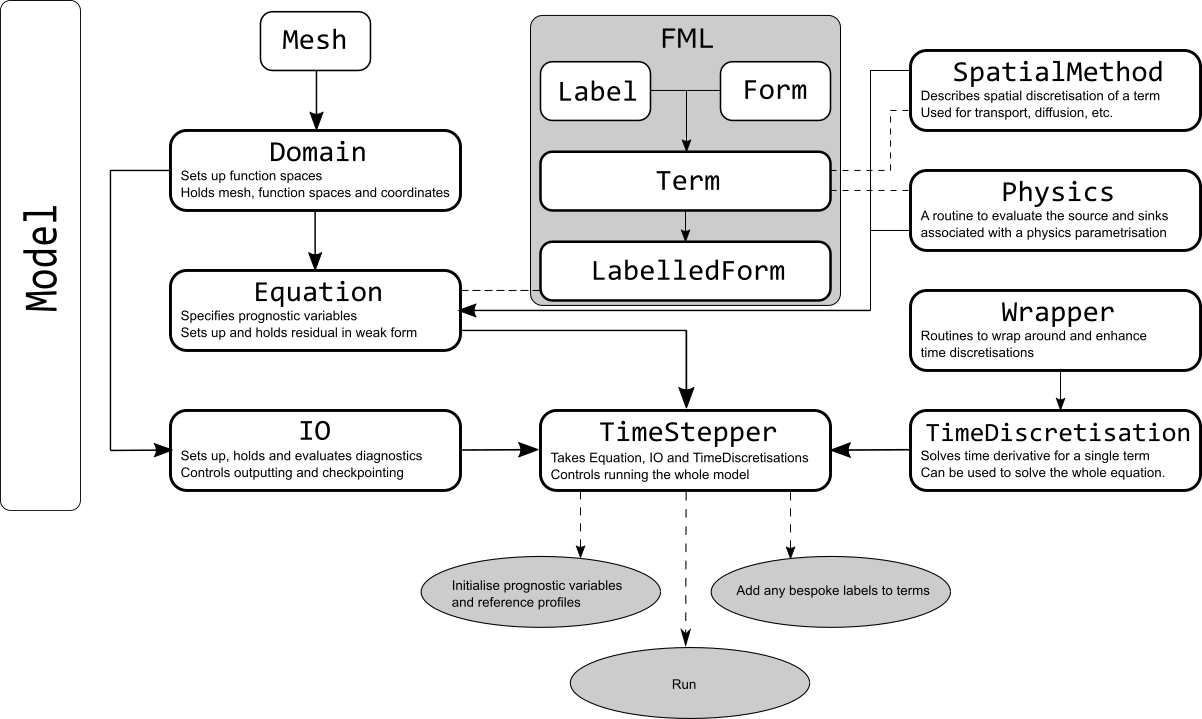
\includegraphics[width=0.8\textwidth]{figures/gusto_schematic.png}}
\end{figure}

\JScomment{This paragraph should refer to the schematic and explain
  all aspects} The Gusto model comprises a domain and a prognostic
equation set. The domain holds the mesh and the finite element
function spaces along with any other information about the space-time
domain such as the coordinates and the timestep. The prognostic
equation sets are each defined in a python class, making use of the
common finite element forms for the transport and difffusion terms to
set up the residual (defined in section \ref{}) in weak form. At this
point, no particular discretisation of the transport or diffusion
forms is specified. This happens in the \texttt{SpatialMethod} class
which can be used to apply the methods described in section \ref{} to
the relevant terms. Any physics source terms, such as **, are added by
calling the \texttt{Physics} class that defines them. The
\texttt{TimeStepper} class contains the definition of the timestepping
procedure and the \texttt{run} method that loops over the
timesteps. It also sets up diagnostic fields and calls the IO as
required. The simplest timeloop class will just apply one time
discretisation method to the equation set but it is common in weather
and climate prediction models to split the different types of terms
and apply a time discretisation separately to each type of term. For
example, the transport and forcing terms might be solved for
separately, such as in **, which enables explicit transport schemes to
be applied to each field. ** something about SIQN structure. Terms
involved in physics parameterisations are evaluated in the appropriate
part of the iteration loop, with physics processes that occur on
`fast' timescales evaluated more frequently and `slower' physics
processes evaluated just once at the end of the timestep. The choice
of where to evaluate the physics processes in the iteration is also
based on the computational cost and the best way to do this is still
an open research question (**ref).

\begin{itemize}
\item what about initialisation and diagnostics?
\end{itemize}

\begin{algorithm}
  \caption{Pseudocode for SIQN timestep loop}\label{alg:SIQN}
  \begin{algorithmic}
    \STATE
  \end{algorithmic}
\end{algorithm}

\begin{itemize}
\item generic example(s) - no FML, just pseudocode for basic
  timestepper, SIQN and split physics
\item lead in to next section... facilitated by FML i.e. timesteppers don't care what equations they're given because forms are labelled
\end{itemize}

\section{Form Manipulation Language}
\label{sec: FML}
The discussion of the time discretisation so far has been general i.e.
not specific to any particular equation set. This is also true of the
implementation of the timestepping schemes, resulting in modular code
where the equations are defined separately from the timestepping
scheme enabling flexibility in applying different timestepping schemes
to different equations. This powerful functionality is facilitated
through the form manipulation language (FML) which is used to
associate a label to each term in the residual form defined in the
equation class. The timestepping methods are then able to reason about
which manipulations to apply to which forms by applying filters that
check for the presence of a label and, optionally, its value. Here we
will describe the objects required to define labels and filters before
illustrating this with some simple examples.

The finite element discretisation of each term in an equation is
represented in Firedrake by a UFL form object. FML defines a
\texttt{Label} object which is used to tag a UFL form to create a
\texttt{Term}, with the intention that the \texttt{Term} represents a
term in the residual. The \texttt{Label} object consists of a name and
an optional value, defaulting to \texttt{True} to indicate the
presence of the label. Labels can be used to tag terms to identify
them as representing particular processes, such as transport, or they
can tag parts of the form. For example, the \texttt{subject} label is
used to tag the \texttt{Function} in the \texttt{ufl.Form} that
represents the prognostic variable, or `subject' of the
equation. These operations are composable, so more than one label can
be attached to a term. The end result of labelling the terms in the
residual is a \texttt{LabelledForm} object that holds a list of terms,
pairing individual \texttt{ufl.Form} objects with FML labels. Labelled
forms can be added together, multiplied by floating point numbers and
extended by adding additional terms. More complex manipulations are
enabled by the \texttt{label\_map} method that provides a way of
filtering the terms in the form based on their labels, applying
different mappings to terms that pass or fail the conditions defined
in the filter. A common operation might be to filter for terms that
have a certain label, such as \texttt{transport}, drop terms that do
not have this label and multiply those that do by the timestep. We
shall demonstrate this in the following example.

\subsection{Example 1: IMEX-Euler applied to the 1d advection diffuction equation}

We demonstrate the use of FML by applying a split timestepping scheme
to the 1D advection diffusion equation
\begin{equation}\label{eq:1dadvdiff}
  q_t + cq_x - \kappa q_{xx} = 0,
\end{equation}
where $q$ is a scalar field, $c$ is the constant transporting velocity
and $\kappa$ is the constant diffusivity. The time discretisation
applies an explicit timestep of forward Euler to the transport term
$cq_x$ and an implicit timestep of backward Euler to the diffusion
term $\kappa q_{xx}$:
\begin{align}
  q^* &= q^n - c \Delta t q_x^n, \label{eq:explicit-advdiff} \\
  q^{n+1} - \kappa \Delta t q_{xx}^{n+1} &= q^*, \label{eq:implicit-advdiff}
\end{align}
where $q^n$ is the value of $q$ at time step $n$, $q^*$ is an
intermediate value for $q$ and $\Delta t$ is the timestep.

We illustrate the use of FML for this example in three steps: 1)
define and label the weak form of the residual, 2) build solvers for
the explicit and implicit systems, 3) run the timestepping loop. Since
the intention of this example is to demonstrate FML rather than the
compatible finite element discretisation, we use the space of piecewise
linear continuous Lagrange polynomials, denoted by $P_1$, for the
finite element discretisation as this greatly simplifies the
forms. The finite element discretisation of equation
\ref{eq:1dadvdiff} is then
\begin{equation}\label{eq:weak-advdiff}
  \int_\Omega vq_t \diff x + c \int_\Omega v q_x \diff x + \kappa \int_\Omega v_x q_x \diff x = 0, \quad \forall v \in P_1,
\end{equation}
where $v\in P_1$ is the test function and the diffusion term has been
integrated by parts.

Listing \ref{lst:define-residual} presents the code to define this
spatial discretisation of the residual with the $P_1$ function space
denoted by \texttt{V}. Here we omit the code that sets up the mesh,
function spaces and parameters $c$ and $\kappa$, although this can be
found in the supplementary materials. The first two lines define the
test function \texttt{v} and function \texttt{q}, corresponding to $v$
and $q$ in equation \ref{eq:weak-advdiff}. The next four lines define
the residual, i.e. the left side of equation \ref{eq:weak-advdiff},
using the FML labels \texttt{time\_derivative}, \texttt{transport} and
\texttt{diffusion} to tag the corresponding terms. The final line
labels the function \texttt{q} as the subject of this residual,
i.e. the prognostic field. Note that the labels used for tagging just
take the UFL form as their argument and their value is simply the
default, \texttt{True}, in contrast to the \texttt{subject} label that
has the value \texttt{q}.

\lstinputlisting[caption={This code defines and labels the residual corresponding to equation \ref{eq:weak-advdiff}}, label={lst:define-residual}, language=python, firstline=24, lastline=31]{code/advection_diffusion_splitting_example.py}

To define the solvers for the explicit and implicit timesteps
(equations \ref{eq:explicit-advdiff} and \ref{eq:implicit-advdiff}),
we need to create UFL forms given by the following equations
\begin{align}
  \label{eq:explicit-advdiff}
  \int_\Omega vq^* \diff x &= \int_\Omega vq^n \diff x - \Delta t c \int_\Omega v q_x^n \diff x, &\quad \forall v \in P^2, \\
  \label{eq:implicit-advdiff}
  \int_\Omega vq^{n+1} \diff x  + \Delta t \kappa \int_\Omega v_x q_x^{n+1} \diff x &= \int_\Omega vq^* \diff x, &\quad \forall v \in P^2.
\end{align}
To do this we use the \texttt{label\_map} method to loop over the
terms in the residual making use of the predefined mappings
\texttt{drop} and \texttt{keep} to either remove or retain the term
based on the value of the filter. This code is given in listings
\ref{lst:define-explicit} and \ref{lst:define-implicit}. In listing
\ref{lst:define-explicit} we create the left and right sides of
equation \ref{eq:explicit-advdiff}. The left side should only contain
the time derivative term so the filter checks if each term has the
label \texttt{time\_derivative}, keeping the one that does and
dropping all others. To make this the left side of a
\texttt{LinearVariationalProblem}, we replace the subject with a trial
function using the predefined \texttt{replace\_subject} function, a
lightweight wrapper around the UFL replace method which extracts the
subject of the term and replaces it with the new expression, in this
case simply a trial function \texttt{q\_trial}. The right side of the
explicit solver has two forms, one coming from the discretisation of
the time derivative and the other from the transport term. Both are
evaluated using the values of $q$ at time step $n$. We build this by
first dropping the diffusion term (line 6) and then multiplying the
terms that do not have the \texttt{time\_derivative} label by $-\Delta
t$ (line 8), where the minus sign is required to move the term from
the left side to the right side. The final step is to replace the
subject with the function \texttt{qn} that holds the values of $q$ at
time step $n$. We can then extract the UFL forms from
\texttt{lhs\_explicit} and \texttt{lhs\_implicit} to create a
\texttt{LinearVariationalProblem} and corresponding
\texttt{LinearVariationalSolver} that, when solved, will put the
result into the function \texttt{qstar}.

\JScomment{Is the
  labelling for the rhs the clearest? maybe we should keep the terms
  that we want rather than assuming that dropping diffusion gives the
  right thing?}

\lstinputlisting[caption={This code defines the solver for the explicit step of the timestepping method i.e. equation \ref{eq:explicit-advdiff}. \texttt{qn} and \texttt{qstar} are Firedrake \texttt{Functions} with \texttt{qn} holding the values of $q$ at time step $n$ and \texttt{qstar} holding the values of $q$ after the explicit solve.}, label={lst:define-explicit}, language=python, firstline=40, lastline=55]{code/advection_diffusion_splitting_example.py}

The implicit solver is defined in a similar way (see listing
\ref{lst:define-implicit}). To create the left side of equation
\ref{eq:implicit-advdiff} we begin with the original residual, drop
the transport term (line 1), multiply all remaining terms that are not
the time derivative by $\Delta t$ (line 3) and replace the subject
with a trial function (line 5). The right side only contains the form
coming from the discretisation of the time derivative (line 7),
evaluated using the result of the explicit solve, \texttt{qstar} (line
9).

\lstinputlisting[caption={This code defines the solver for the implicit step of the timestepping method i.e. equation \ref{eq:implicit-advdiff}. \texttt{qstar} and \texttt{qnp1} are Firedrake \texttt{Functions} with \texttt{qstar} holding the values after the explicit solve and \texttt{qnp1} holding the values of $q$ at after the implicit solve.}, label={lst:define-implicit}, language=python, firstline=57, lastline=71]{code/advection_diffusion_splitting_example.py}

The final part of the code is the time loop which calls the solve
method of first the explicit solver and then the implicit solver, see
listing \ref{lst:timeloop}. In practice, the code in listings
\ref{lst:define-explicit}-\ref{lst:define-implicit} would be in a
function that could be applied to any residual labeled with the
appropriate labels.

\lstinputlisting[caption={This code is the timeloop implementing the scheme defined in equations \ref{eq:explicit-advdiff}-\ref{eq:implicit-advdiff} using the solvers defined in listings \ref{lst:define-explicit}-\ref{lst:define-implicit}.}, label={lst:timeloop}, language=python, firstline=73, lastline=79]{code/advection_diffusion_splitting_example.py}

This simple example demonstrates the power of manipulating the terms
in the equation based on the presence or absence of certain
labels. The full strength of FML becomes even more apparant when we
exploit information stored in the label value. We use this in two
important situations in Gusto. The first situation is when we need to
evaluate source terms that come from physics schemes. The second
situation is when we require a linearisation of the residual, for
example when applying a quasi-Newton method to solve the full
nonlinear equations or when testing a new algorithm on the linear
equations. We illustrate both situations in the following two
examples.

\subsection{Example 2: Sequential splitting for an idealised chemistry-transport problem} \label{sec:seq splitting}



\subsection{Example 3: Quasi-Newton } \label{sec:siqn}



\section{Results}
\label{sec: results}
The aim of this section is to present a selection of results that
showcase the tools available in Gusto, such as the choice of grids,
HDiv element families, order of finite element spaces, different
spatial discretisation options and timestepping schemes.
As these options can be combined in so many ways, it is only possible to present results from a tiny fraction of the configurations.
We have chosen to use a selection from the hierarchy of standard test cases that span the stages of development of dynamical cores.
Although we do include some results here that demonstrate the numerical properties of certain configurations, the purpose of this section is not to provide a rigorous verification of any particular choice of discretisation. Such results are demonstrated elsewhere, for instance \citet{bendall2020compatible} or \citet{hartney2025exploring}.
The settings used for each result from this section are detailed in Appendix \ref{sec:appendix}.

\subsection{Terminator Toy chemistry}
The first results use the ``Terminator Toy'' test of \citet{lauritzen2015terminator}, which involves the transport of two coupled tracers $X$ and $X_2$ on the surface of a sphere.
The chemicals interact such that the sum $m_T=m_X+2m_{X_2}$ should be preserved, where $m_X$ and $m_{X_2}$ are the mixing ratios of the individual chemicals.
When positivity or monotonicity limiters are applied to the numerical transport scheme, this may break the correlation between the two species which will be highlighted by this test.
This test is also a demonstration of simple ``physics-dynamics coupling'', as the conversion term between the species can be handled separately from the transport terms. \\
\\
For this test, we use the DG upwind scheme described in Section \ref{sec:transport} to transport the species on an icosahedral sphere mesh, and apply the vertex-based limiter of \citet{kuzmin2010vertex}.
The term describing the chemical reaction is separated from the transport term using a simple sequential splitting, as described in Section \ref{sec:seq splitting}. \\
\\
Figure \ref{fig:terminator} shows the mixing ratios of the two individual species at the initial time and following a single rotation around the sphere by a deformational flow.
The change in the sum of the species is also displayed, with differences from zero remaining close to machine precision, which demonstrates that this transport scheme does preserve the correlation between the tracers. 

\begin{figure}[htp!]
\centering
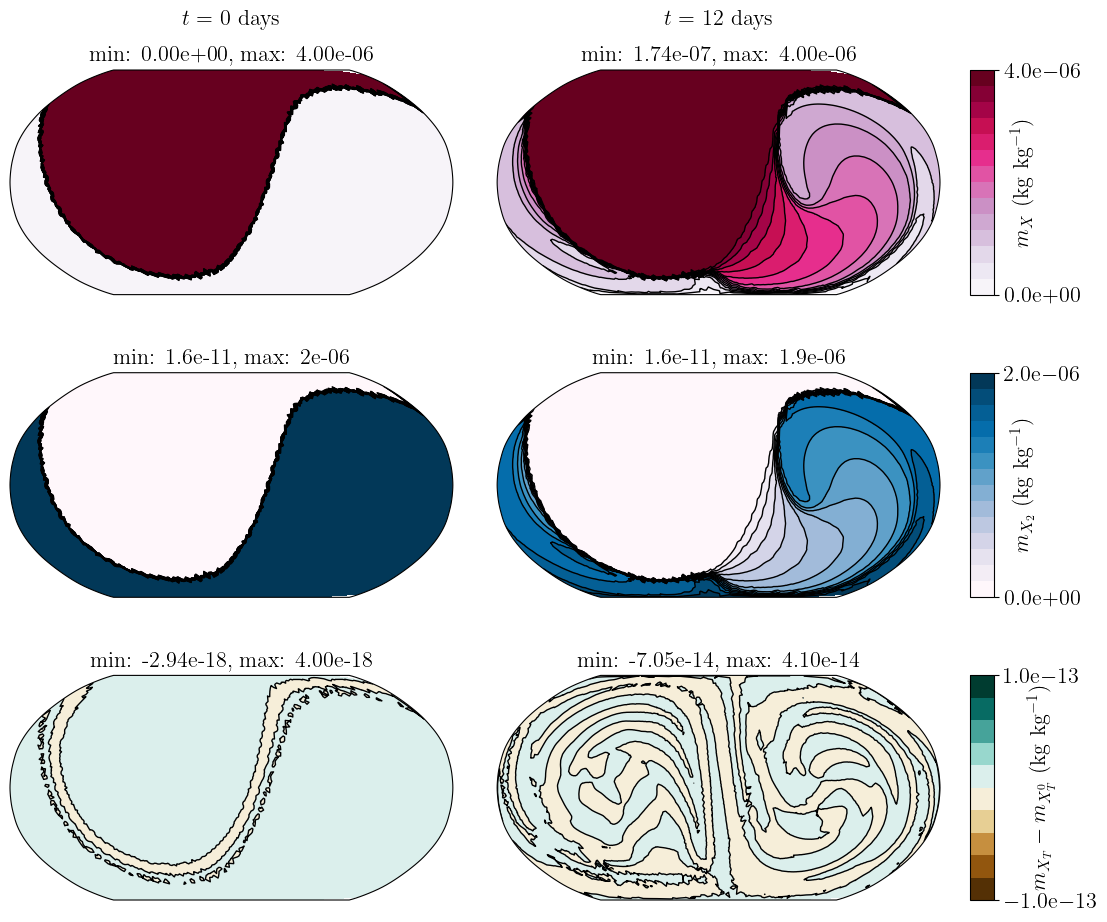
\includegraphics[width=0.9\textwidth]{figures/terminator_toy.png}
\caption{The evolution of the chemical species from the ``Terminator Toy'' test of \citet{lauritzen2015terminator}.
The fields at the initial time are shown on the left, and at the final time ($t=12$ days) which follows a single revolution around the sphere by a deformational flow.
The bottom row shows the change in the total $m_T=m_X+2m_{X_2}$ from the initial time, which remains very close to zero.}
\label{fig:terminator}
\end{figure}

\subsection{Shallow water}
The standard suite of shallow water test cases originally proposed in
\citet{williamson1992standard} provides a common starting point for
testing new discretisations. This test suite is often augmented by
the unstable barotropic jet described in
\citet{galewsky2004initial}. \\
\\
Here we present two sets of convergence results for a variety of configurations measured using the steady state geostrophic balanced flow (test case 2 from
\citet{williamson1992standard}) with the linear shallow water equations, as used in \citet{weller2012computational}.
Figure \ref{fig:sw_convergence} shows the spatial convergence for a number of choices of finite element for the prognostic variables, using a Trapezium Rule discretisation (also known as Crank-Nicolson).
It also shows the temporal convergence for a range of timestepping schemes using the 1st order Raviart-Thomas elements on quadrilateral cells. 
\textcolor{red}{Once the test has been completed, come back to edit what we say here about convergence!} \\
\\
We show results from the unstable jet of \citet{galewsky2004initial} in Figure \ref{fig:galewsky}, using the non-linear shallow water equations.
These results use the Semi-Implicit Quasi-Newton timestepper described in Section \ref{sec:siqn}, and compare the first-order RT elements on a cubed-sphere mesh with the first-order BDM elements on an icosahedral-sphere.

\begin{figure}[htp!]
\centering
\includegraphics[width=0.9\textwidth]{}
\caption{Convergence results using the linear shallow water equations with the steady geostrophic flow of \citet{williamson1992standard}.
(Left) the spatial convergence of a number of orders and families of finite element, all using the same timestepper. (Right) the temporal convergence of different timesteppers, all using the same spatial discretisation.}
\label{fig:sw_convergence}
\end{figure}

\begin{figure}[htp!]
\centering
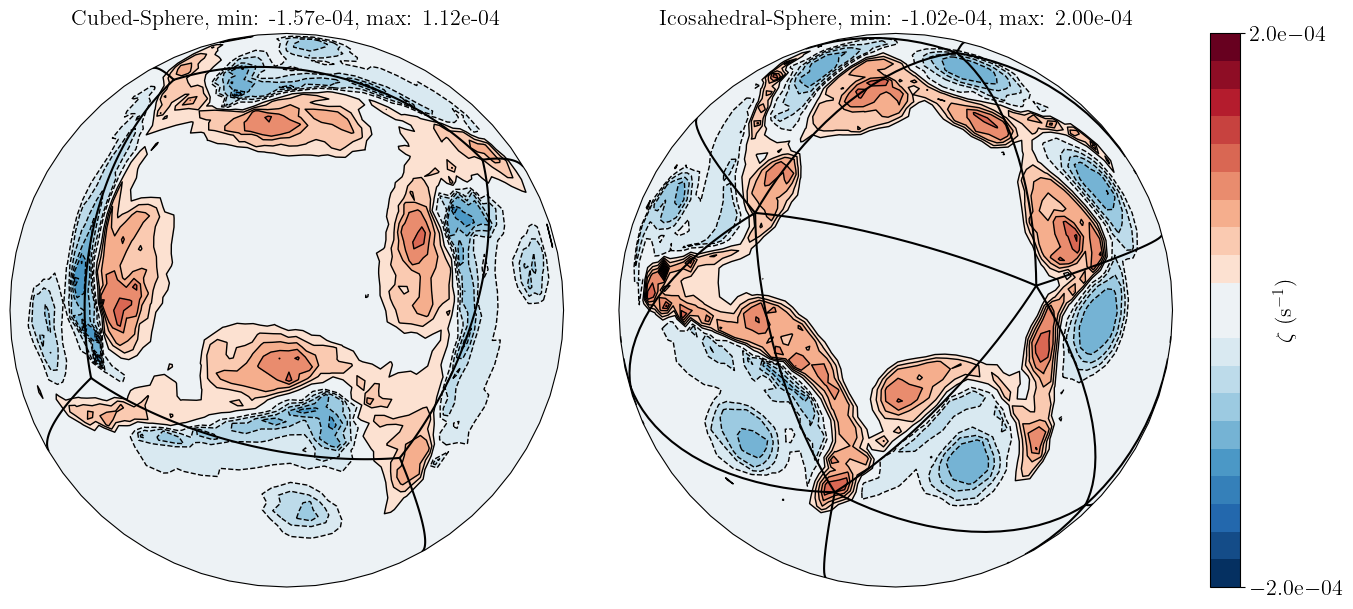
\includegraphics[width=0.9\textwidth]{figures/galewsky_jet.png}
\caption{A view of the relative vorticity around the North pole at day 6 of a simulation of the Galewsky jet test case. (Left) the RT1 elements on a cubed-sphere mesh. (Right) the BDM1 elements on an icosahedral-sphere mesh. Both cases use the Semi-Implicit Quasi-Newton timestepper. The edges of the panels of the cube and icosahedron are highlighted.}
\label{fig:galewsky}
\end{figure}

\subsection{Compressible Euler equations}
We have also implemented many of the standard test cases for the non-hydrostatic compressible Euler equations that are used in modern weather and climate models.
In this section we show results from a small selection of these, which demonstrate different domains in which these methods work.
Throughout this section we use the Semi-Implicit Quasi-Newton timestepper.
 \\
\\
The first test is the falling density current of \citet{straka1993numerical} in a vertical slice. This test involves the addition of diffusion to both the potential temperature and velocity equations.
Figure \ref{fig:straka} shows the final potential temperature field for simulations using the lowest-order and next-to-lowest order finite elements on the vertical slice.
The lowest-order methods require the transport and diffusion terms to use the ``recovered'' scheme of \citet{bendall2019recovered} to attain second-order accuracy. 
\\
\begin{figure}[htp!]
\centering
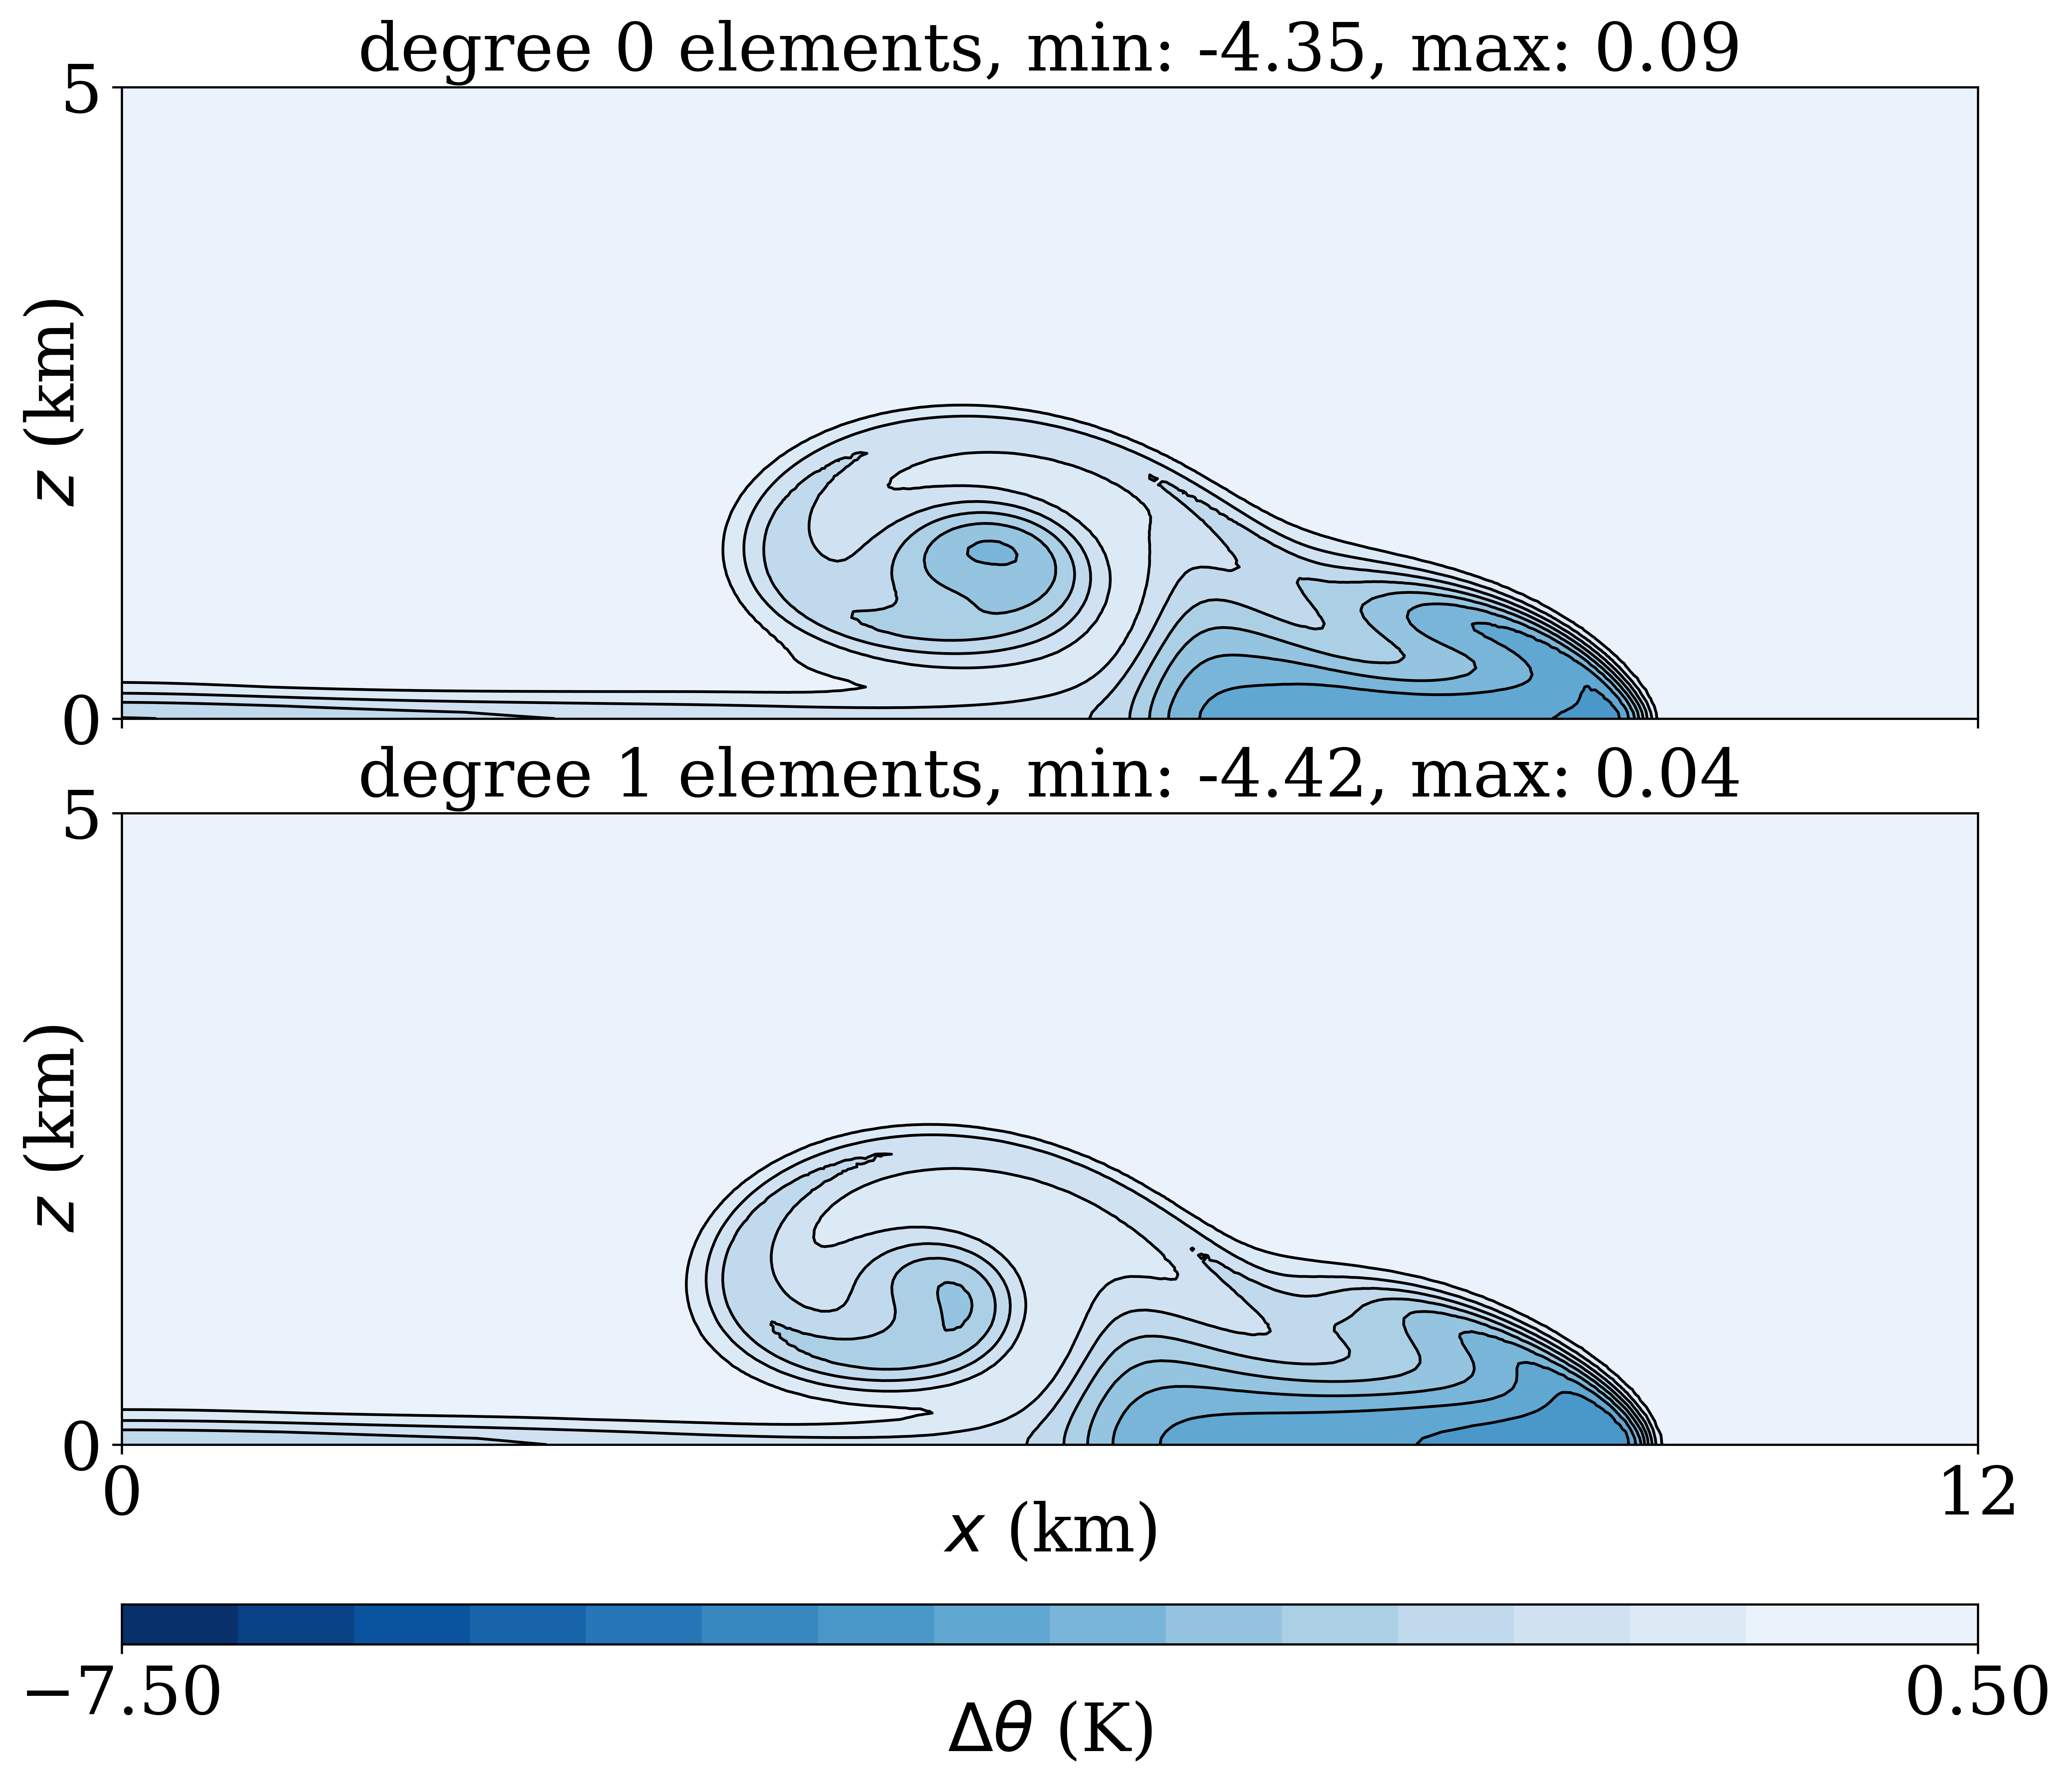
\includegraphics[width=0.8\textwidth]{figures/straka.png}
\caption{The potential temperature field after 900 s from the falling density current test of \citet{straka1993numerical}. (Top) with the lowest-order finite elements, and (bottom) with the next-to-lowest-order finite elements.
}
\label{fig:straka}
\end{figure}
\\
To demonstrate the use of moist physics parametrisations, we use a moist three-dimensional rising thermal simulation in an extruded doubly-periodic plane.
The initial conditions are those of \citet{bendall2020compatible}, which is an extension of the dry case of \citet{kelly2012continuous} and \citet{melvin2019mixed}.
A cross-sections of the final equivalent potential temperature field is shown in Figure \ref{fig:3d_bubble}.
As in the two-dimensional test of \citet{bryan2002benchmark}, the atmosphere is saturated and cloudy everywhere, so that the moist processes are active in the whole domain.
A simple saturation adjustment parametrisation is used, with the details described in \citet{bendall2020compatible}.
\\
\begin{figure}[htp!]
\centering
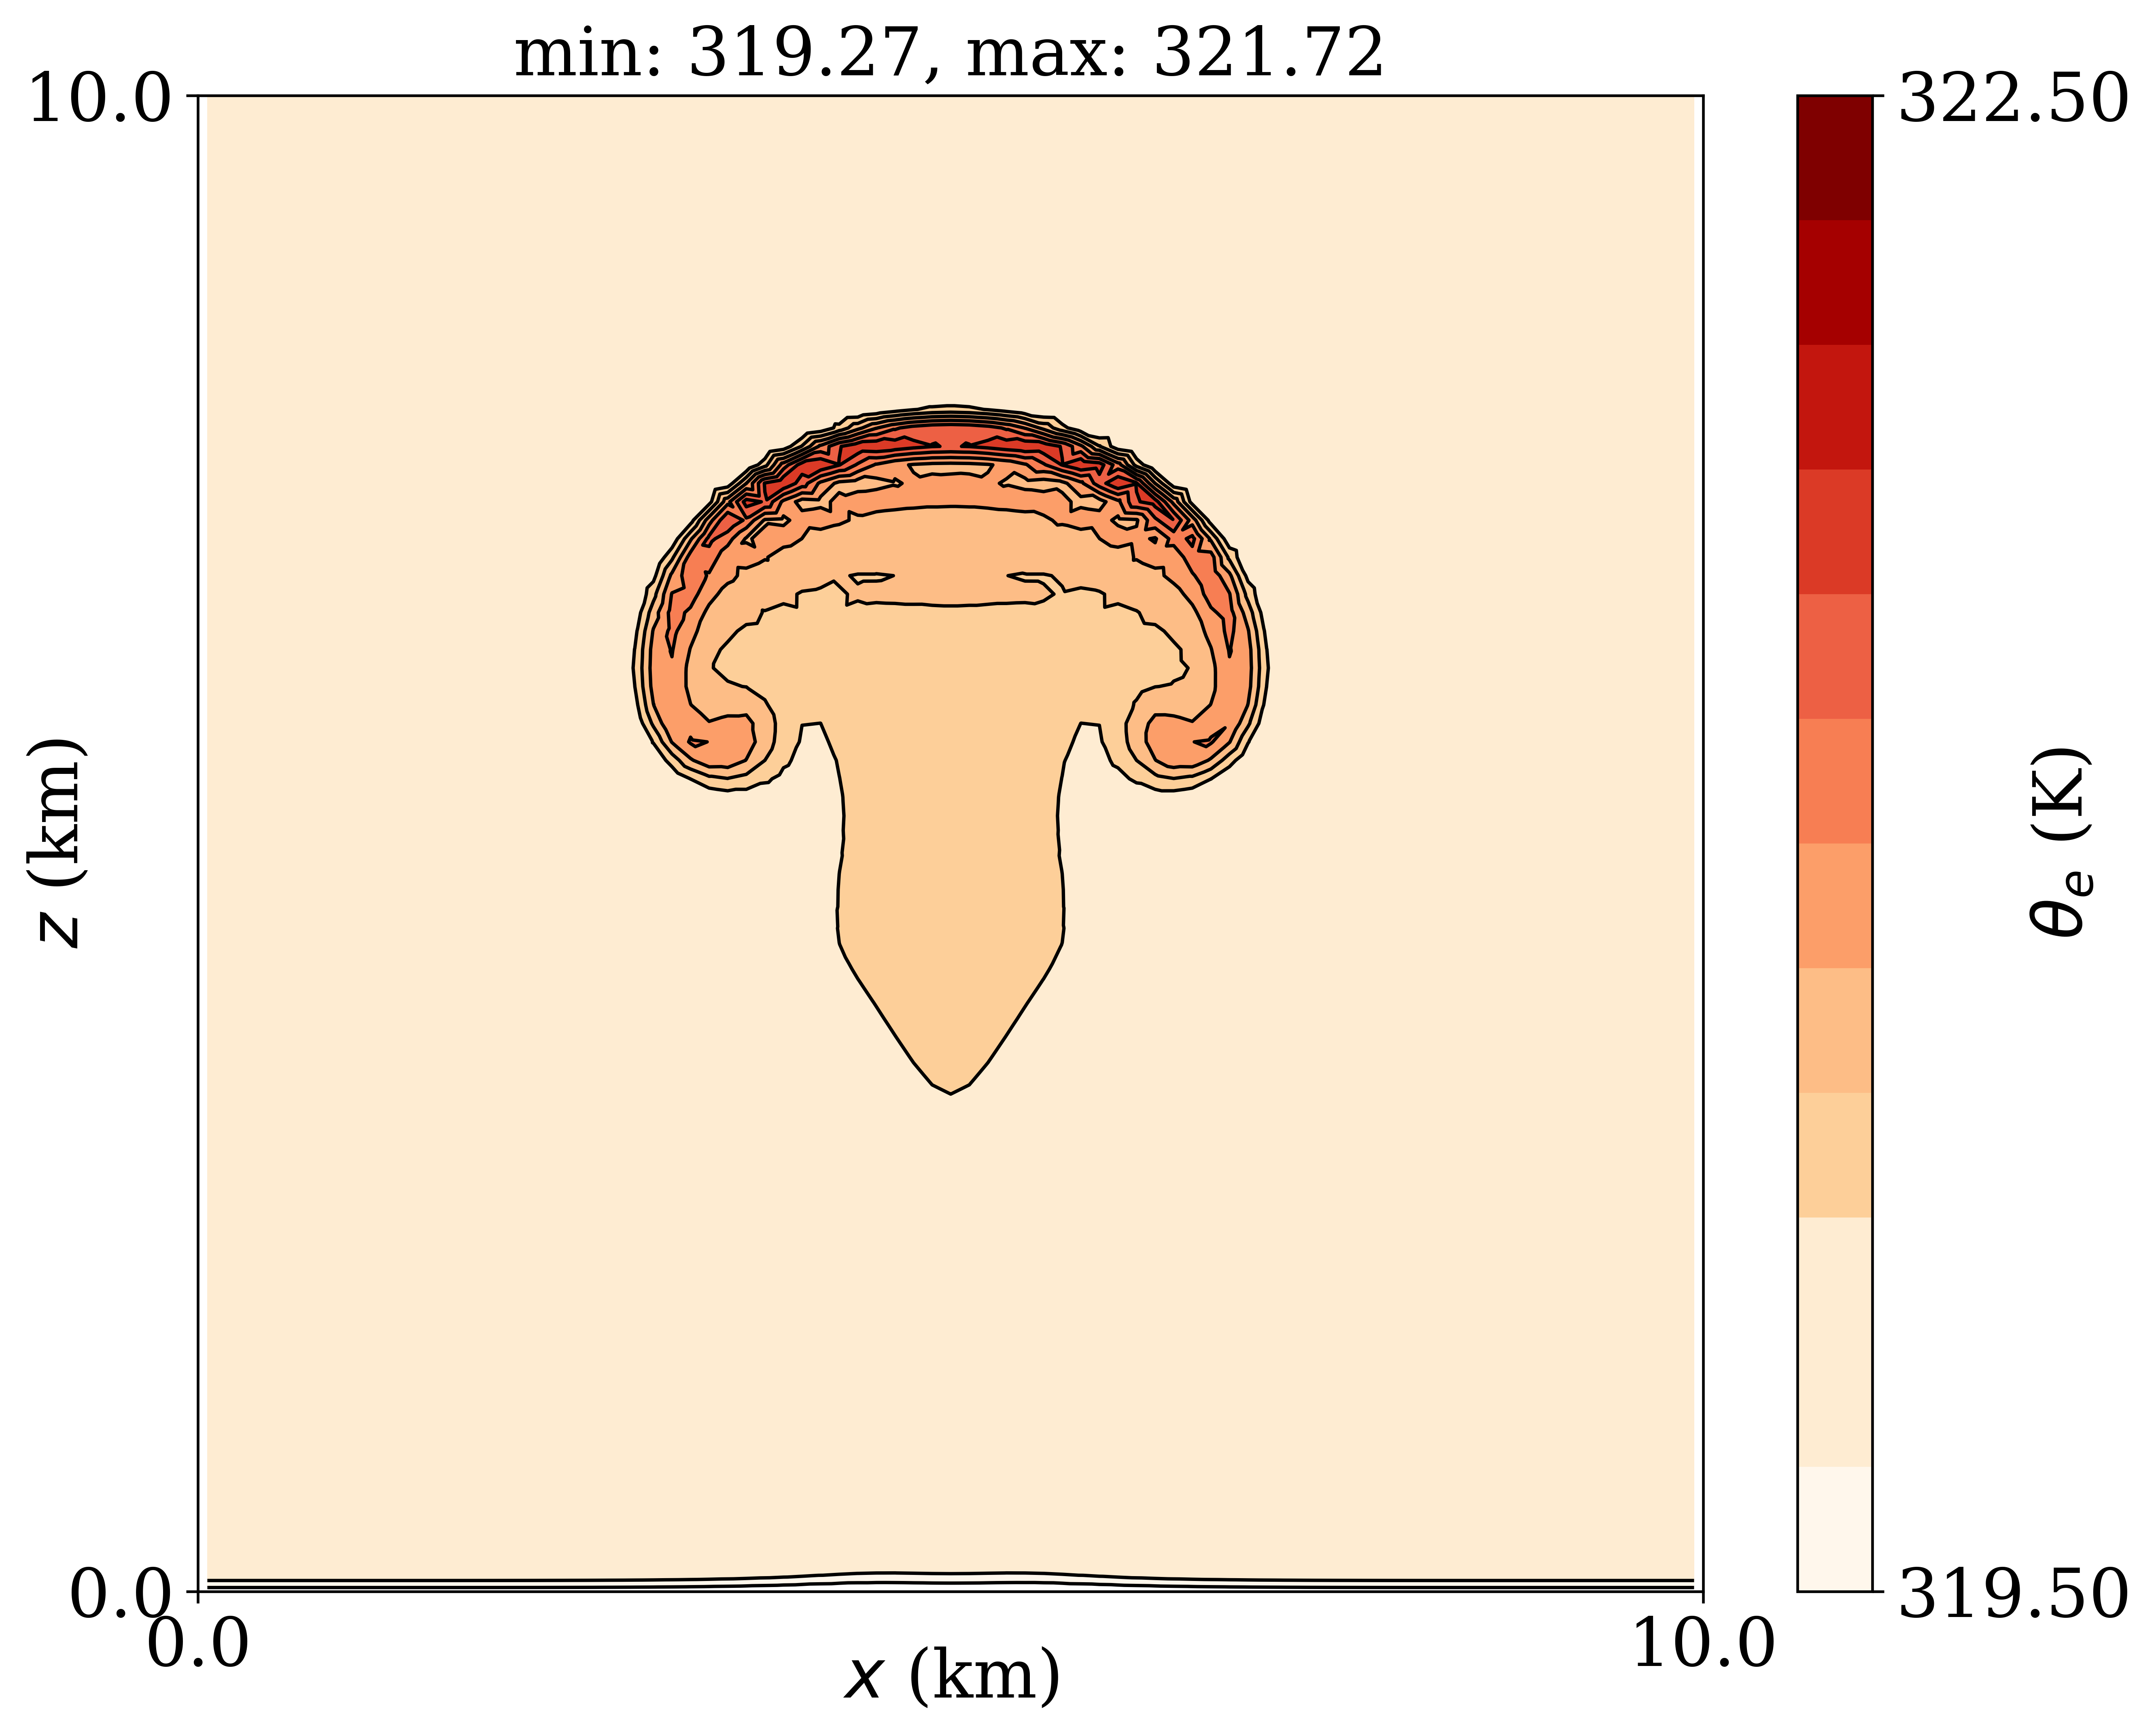
\includegraphics[width=0.48\textwidth]{figures/moist_3d_bubble.png}
\caption{Vertical cross-section of the final equivalent potential temperature field from the three-dimensional moist rising thermal test.
}
\label{fig:3d_bubble}
\end{figure}
\\
Our final test case is the deep baroclinic wave of \citet{ullrich2014proposed} on the sphere.
An initial state in thermal wind balance is perturbed to produce a mid-latitude baroclinic instability, providing a flow that is typical of those found in numerical weather prediction.
The surface pressure and temperature fields after 10 days are shown in Figure \ref{fig:baroclinic}, which compare well with those in \citet{melvin2024mixed} and demonstrate that our methods can replicate results from the literature.

\begin{figure}[htp!]
\centering
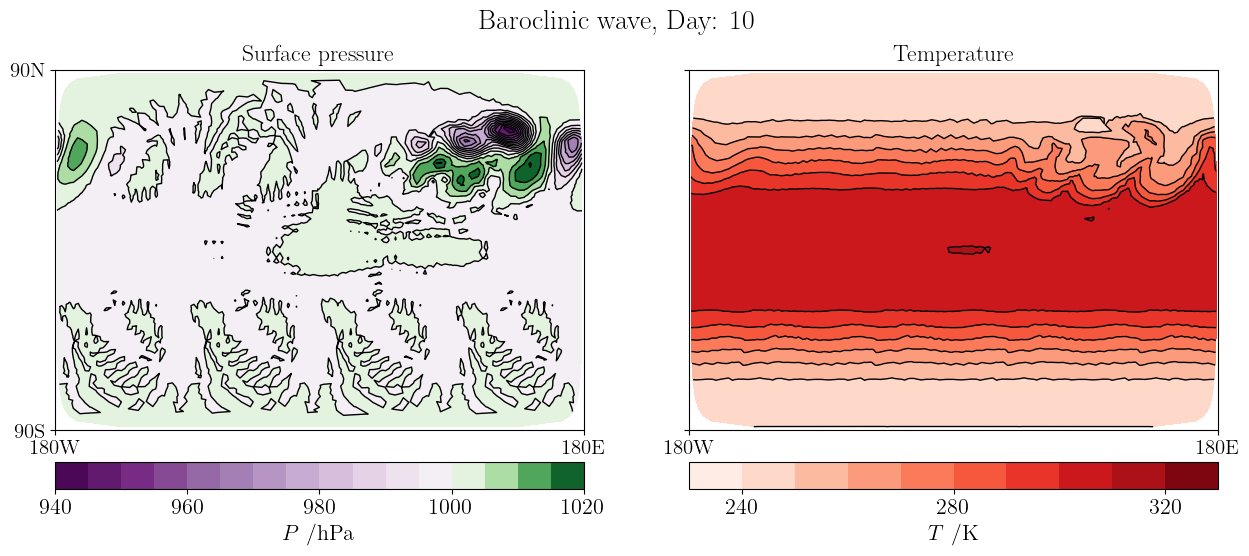
\includegraphics[width=0.9\textwidth]{figures/baroclinic_wave_lonlat.png}
\caption{The surface pressure and temperature after 10 days of a deep baroclinic wave simulation on the cubed-sphere.}
\label{fig:baroclinic}
\end{figure}

\section{Summary}
\label{sec: summary}


\conclusions  %% \conclusions[modified heading if necessary]
TEXT

%% The following commands are for the statements about the availability of data sets and/or software code corresponding to the manuscript.
%% It is strongly recommended to make use of these sections in case data sets and/or software code have been part of your research the article is based on.

\codeavailability{TEXT} %% use this section when having only software code available


\dataavailability{TEXT} %% use this section when having only data sets available


\codedataavailability{TEXT} %% use this section when having data sets and software code available


\sampleavailability{TEXT} %% use this section when having geoscientific samples available


\videosupplement{TEXT} %% use this section when having video supplements available


\appendix
\section{Test Case Settings}  \label{sec:appendix}  %% Appendix A
Here we summarise the configuration details for the test cases used to produce the results in Section \ref{sec: results}.

\begin{sidewaystable*}[tbp!]
\caption{Details of the configurations used for the test cases in Section \ref{sec: results}.}
\begin{tabular}{l|ccccccc}
\tophline
Test Case & Equation Set & Timestepper & Finite Elements & \begin{tabular}{@{}c@{}}Horizontal \\ Mesh\end{tabular} & \begin{tabular}{@{}c@{}}Number \\ of  \ Layers\end{tabular} & Time step & Final Time \\
\middlehline
Terminator Toy & \begin{tabular}{@{}c@{}}Tracer transport \\ with chemistry\end{tabular} & Sequential Splitting & BDM1 & I16 & None & 450 s & 12 days \\
Steady Geostrophic Flow & Linear Shallow Water & Multiple & BDM1 & I32 & None & ?? & 1 day \\
Steady Geostrophic Flow & Linear Shallow Water & Trapezium Rule & Multiple & ?? & None & ?? & 1 day \\
Unstable Jet & Shallow Water & SIQN & BDM1 and RT1 & I64 and C100 & None & 150 s & 6 days \\
Density Current & Compressible Euler & SIQN & RT0 and RT1 & 100 m and 200 m & 64 and 32 & 1 s & 900 s \\
Rising Thermal & Moist Compressible Euler & SIQN & RT1 & $\Delta x = \Delta y = \frac{10}{81}$ km & 81 & 2 s & 1000 s \\
Baroclinic Wave & Compressible Euler & SIQN & RT1 & C32 & 15 & 900 s & 10 days
\bottomhline
\end{tabular}
\belowtable{Notation: RT$x$ refers to the de Rham complex that uses the Raviart-Thomas elements on quadrilateral cells for the HDiv function space, and results in an $x$-th order polynomials for the $L_2$ space. Similarly, BDM$x$ refers to the Brezzi-Douglas-Marini de Rham complex on triangular cells.
SIQN denotes the Semi-Implicit Quasi-Newton timestepper described in Section \ref{sec:siqn}. When describing horizontal meshes of the sphere, I$y$ and C$y$ correspond to icosehedral-sphere and cubed-sphere meshes with $y$ cells per edge of the icosahedron or cube panel.}% Table Footnotes
\end{sidewaystable*}

\subsection{}     %% Appendix A1, A2, etc.


\noappendix       %% use this to mark the end of the appendix section. Otherwise the figures might be numbered incorrectly (e.g. 10 instead of 1).

%% Regarding figures and tables in appendices, the following two options are possible depending on your general handling of figures and tables in the manuscript environment:

%% Option 1: If you sorted all figures and tables into the sections of the text, please also sort the appendix figures and appendix tables into the respective appendix sections.
%% They will be correctly named automatically.

%% Option 2: If you put all figures after the reference list, please insert appendix tables and figures after the normal tables and figures.
%% To rename them correctly to A1, A2, etc., please add the following commands in front of them:

\appendixfigures  %% needs to be added in front of appendix figures

\appendixtables   %% needs to be added in front of appendix tables

%% Please add \clearpage between each table and/or figure. Further guidelines on figures and tables can be found below.



\authorcontribution{TEXT} %% this section is mandatory

\competinginterests{TEXT} %% this section is mandatory even if you declare that no competing interests are present

\disclaimer{TEXT} %% optional section

\begin{acknowledgements}
TEXT
\end{acknowledgements}




%% REFERENCES

%% The reference list is compiled as follows:

%% \begin{thebibliography}{}

%% \bibitem[AUTHOR(YEAR)]{LABEL1}
%% REFERENCE 1

%% \bibitem[AUTHOR(YEAR)]{LABEL2}
%% REFERENCE 2

%% \end{thebibliography}

%% Since the Copernicus LaTeX package includes the BibTeX style file copernicus.bst,
%% authors experienced with BibTeX only have to include the following two lines:
%%
\bibliographystyle{copernicus}
\bibliography{references.bib}
%%
%% URLs and DOIs can be entered in your BibTeX file as:
%%
%% URL = {http://www.xyz.org/~jones/idx_g.htm}
%% DOI = {10.5194/xyz}


%% LITERATURE CITATIONS
%%
%% command                        & example result
%% \citet{jones90}|               & Jones et al. (1990)
%% \citep{jones90}|               & (Jones et al., 1990)
%% \citep{jones90,jones93}|       & (Jones et al., 1990, 1993)
%% \citep[p.~32]{jones90}|        & (Jones et al., 1990, p.~32)
%% \citep[e.g.,][]{jones90}|      & (e.g., Jones et al., 1990)
%% \citep[e.g.,][p.~32]{jones90}| & (e.g., Jones et al., 1990, p.~32)
%% \citeauthor{jones90}|          & Jones et al.
%% \citeyear{jones90}|            & 1990



%% FIGURES

%% When figures and tables are placed at the end of the MS (article in one-column style), please add \clearpage
%% between bibliography and first table and/or figure as well as between each table and/or figure.

% The figure files should be labelled correctly with Arabic numerals (e.g. fig01.jpg, fig02.png).


%% ONE-COLUMN FIGURES

%%f
%\begin{figure}[t]
%\includegraphics[width=8.3cm]{FILE NAME}
%\caption{TEXT}
%\end{figure}
%
%%% TWO-COLUMN FIGURES
%
%%f
%\begin{figure*}[t]
%\includegraphics[width=12cm]{FILE NAME}
%\caption{TEXT}
%\end{figure*}
%
%
%%% TABLES
%%%
%%% The different columns must be seperated with a & command and should
%%% end with \\ to identify the column brake.
%
%%% ONE-COLUMN TABLE
%
%%t
%\begin{table}[t]
%\caption{TEXT}
%\begin{tabular}{column = lcr}
%\tophline
%
%\middlehline
%
%\bottomhline
%\end{tabular}
%\belowtable{} % Table Footnotes
%\end{table}
%
%%% TWO-COLUMN TABLE
%
%%t
%\begin{table*}[t]
%\caption{TEXT}
%\begin{tabular}{column = lcr}
%\tophline
%
%\middlehline
%
%\bottomhline
%\end{tabular}
%\belowtable{} % Table Footnotes
%\end{table*}
%
%%% LANDSCAPE TABLE
%
%%t
%\begin{sidewaystable*}[t]
%\caption{TEXT}
%\begin{tabular}{column = lcr}
%\tophline
%
%\middlehline
%
%\bottomhline
%\end{tabular}
%\belowtable{} % Table Footnotes
%\end{sidewaystable*}
%
%
%%% MATHEMATICAL EXPRESSIONS
%
%%% All papers typeset by Copernicus Publications follow the math typesetting regulations
%%% given by the IUPAC Green Book (IUPAC: Quantities, Units and Symbols in Physical Chemistry,
%%% 2nd Edn., Blackwell Science, available at: http://old.iupac.org/publications/books/gbook/green_book_2ed.pdf, 1993).
%%%
%%% Physical quantities/variables are typeset in italic font (t for time, T for Temperature)
%%% Indices which are not defined are typeset in italic font (x, y, z, a, b, c)
%%% Items/objects which are defined are typeset in roman font (Car A, Car B)
%%% Descriptions/specifications which are defined by itself are typeset in roman font (abs, rel, ref, tot, net, ice)
%%% Abbreviations from 2 letters are typeset in roman font (RH, LAI)
%%% Vectors are identified in bold italic font using \vec{x}
%%% Matrices are identified in bold roman font
%%% Multiplication signs are typeset using the LaTeX commands \times (for vector products, grids, and exponential notations) or \cdot
%%% The character * should not be applied as mutliplication sign
%
%
%%% EQUATIONS
%
%%% Single-row equation
%
%\begin{equation}
%
%\end{equation}
%
%%% Multiline equation
%
%\begin{align}
%& 3 + 5 = 8\\
%& 3 + 5 = 8\\
%& 3 + 5 = 8
%\end{align}
%
%
%%% MATRICES
%
%\begin{matrix}
%x & y & z\\
%x & y & z\\
%x & y & z\\
%\end{matrix}
%
%
%%% ALGORITHM
%
%\begin{algorithm}
%\caption{...}
%\label{a1}
%\begin{algorithmic}
%...
%\end{algorithmic}
%\end{algorithm}
%
%
%%% CHEMICAL FORMULAS AND REACTIONS
%
%%% For formulas embedded in the text, please use \chem{}
%
%%% The reaction environment creates labels including the letter R, i.e. (R1), (R2), etc.
%
%\begin{reaction}
%%% \rightarrow should be used for normal (one-way) chemical reactions
%%% \rightleftharpoons should be used for equilibria
%%% \leftrightarrow should be used for resonance structures
%\end{reaction}
%
%
%%% PHYSICAL UNITS
%%%
%%% Please use \unit{} and apply the exponential notation


\end{document}
